%%%%%%%%%%%%%%%%%%%%%%%%%%%%%% -*- Mode: Latex -*- %%%%%%%%%%%%%%%%%%%%%%%%%%%%
%% 10-05.tex --      IEEE Smart Grid Comm paper
%% Author          : Philip Johnson
%% Created On      : Mon Sep 23 11:52:28 2002
%% Last Modified By: Philip Johnson
%% Last Modified On: Mon Apr 12 14:01:35 2010
%%%%%%%%%%%%%%%%%%%%%%%%%%%%%%%%%%%%%%%%%%%%%%%%%%%%%%%%%%%%%%%%%%%%%%%%%%%%%%%
%%   Copyright (C) 2009 Philip Johnson
%%%%%%%%%%%%%%%%%%%%%%%%%%%%%%%%%%%%%%%%%%%%%%%%%%%%%%%%%%%%%%%%%%%%%%%%%%%%%%%
%% 

%% Home page: http://www.ieee-smartgridcomm.org/submission.html

%% Must submit to one of the 12 symposia:
%% http://www.ieee-smartgridcomm.org/symposia.html

%% It appears that this is the most relevant symposia:
%% http://www.ieee-smartgridcomm.org/hibfn.html

%% For ``peer review mode'', do:
%%   \documentclass[conference,compsoc,peerreview]{IEEEtran}
%% and
%%   \IEEEpeerreviewmaketitle  (after the abstract).

%\documentclass[conference,compsoc,peerreview]{IEEEtran}
\documentclass[conference,compsoc]{IEEEtran}
\usepackage[final]{graphicx}
\usepackage{cite}
\usepackage{url}
% uncomment the % away on next line to produce the final camera-ready version
% and uncomment the \thispagestyle{empty} following \maketitle
%\pagestyle{empty}

\begin{document}

\title{WattDepot: An open source software ecosystem for enterprise-scale
  energy data collection, storage, analysis, and visualization}

\author{Robert S. Brewer\\
        Philip M. Johnson \\
\em     Collaborative Software Development Laboratory \\
        Department of Information and Computer Sciences \\
        University of Hawai'i \\
        Honolulu, HI 96822 \\
        \{rbrewer,johnson\}@hawaii.edu \\
}


\maketitle
%\IEEEpeerreviewmaketitle
%\thispagestyle{empty}

\begin{abstract}  % 200 words
  WattDepot is an open source, ethernet-based, service-oriented framework 
  for collection, storage, analysis, and visualization of energy data.
  WattDepot differs from other energy management solutions in one or more
  of the following ways: it is not tied to any specific metering
  technology; it provides high-level support for meter aggregation and data
  interpolation; it supports carbon intensity analysis; it is
  architecturally decoupled from the underlying storage technology; it
  supports both hosted and local energy services; it can provide near-real
  time data collection and feedback; and the software is open source and
  freely available.  In this paper, we introduce the framework, provide
  examples of its use, and discuss its application to research and
  understanding of the Smart Grid.
\end{abstract}


\section{Introduction}
\label{sec:intro}

Recent interest in the Smart Grid has produced a wide variety of proposed
``open'' standards and technologies for energy data collection, storage,
and analysis.  Some prominent approaches include cloud-based services like
Google PowerMeter \cite{GooglePowerMeter} and Microsoft Hohm
\cite{MicrosoftHohm}, ``interoperable'' protocols and networking approaches
like Smart Energy 2.0 \cite{SmartEnergy2.0} and GridRouter Ecosystem
\cite{GridRouterEcosystem}, smart grid standards like IEEE SCC21
\cite{IEEESCC21} and Oasis Blue \cite{OasisBlue}, extensible energy
management devices like Control4's EMS 100 \cite{EMS100}.  There are also
``open source'' hardware platforms, such as OSHAN \cite{OSHAN}, and open
source software solutions for phasor data such as OpenPDC \cite{OpenPDC}.

For our research on behavioral change among energy consumers in a building
or home environment, we need a way to: (a) collect energy data from a
variety of meters with the possibility of near-real time (5-10 second)
feedback, (b) store the results in an internet-accessable repository; (c)
perform basic analyses on the raw data including aggregation and
interpolation, and (d) visualize the raw and processed data in a variety of
ways, including tables, gauges, trend lines, geo maps, heat maps, and so forth.

Unfortunately, we find that none of the current ``open'' technologies
satisfy these seemingly simple requirements. Either the technology is
designed for a specific brand of meter, such as the EMS 100, or it does not
support near-real time feedback (such as Google PowerMeter and Microsoft
Hohm), or it focuses on utility issues (OpenPDC), or it focusses on
wire-level or hardware concerns (OSHAN, GridRouter Ecosystem).

Rather than implement a special purpose solution for our research, we
decided to leverage our prior experience in open source software
engineering measurement systems to design and implement an open source,
extensible, service-oriented framework for energy data collection, storage,
analysis, and visualization. Our framework, called WattDepot, consists of
three kinds of services:

\begin{itemize}
\item WattDepot {\em sensors}, each customized for a particular brand of
energy meter.  A sensor requests data from a meter according to the meter's
protocol, then sends it to a WattDepot repository for storage.

\item WattDepot {\em repositories}, which implement a REST \cite{REST} API
for accepting energy data sent from sensors and providing this sensor data
(or analyses based upon the data) to WattDepot clients.

\item WattDepot {\em clients}, which request data from WattDepot
repositories and either visualize the data or analyses directly to users or
provide the data to higher level energy services.
\end{itemize}

Figure \ref{fig:architecture} illustrates the architecture of the system.

\begin{figure*}[!th]
  \center
  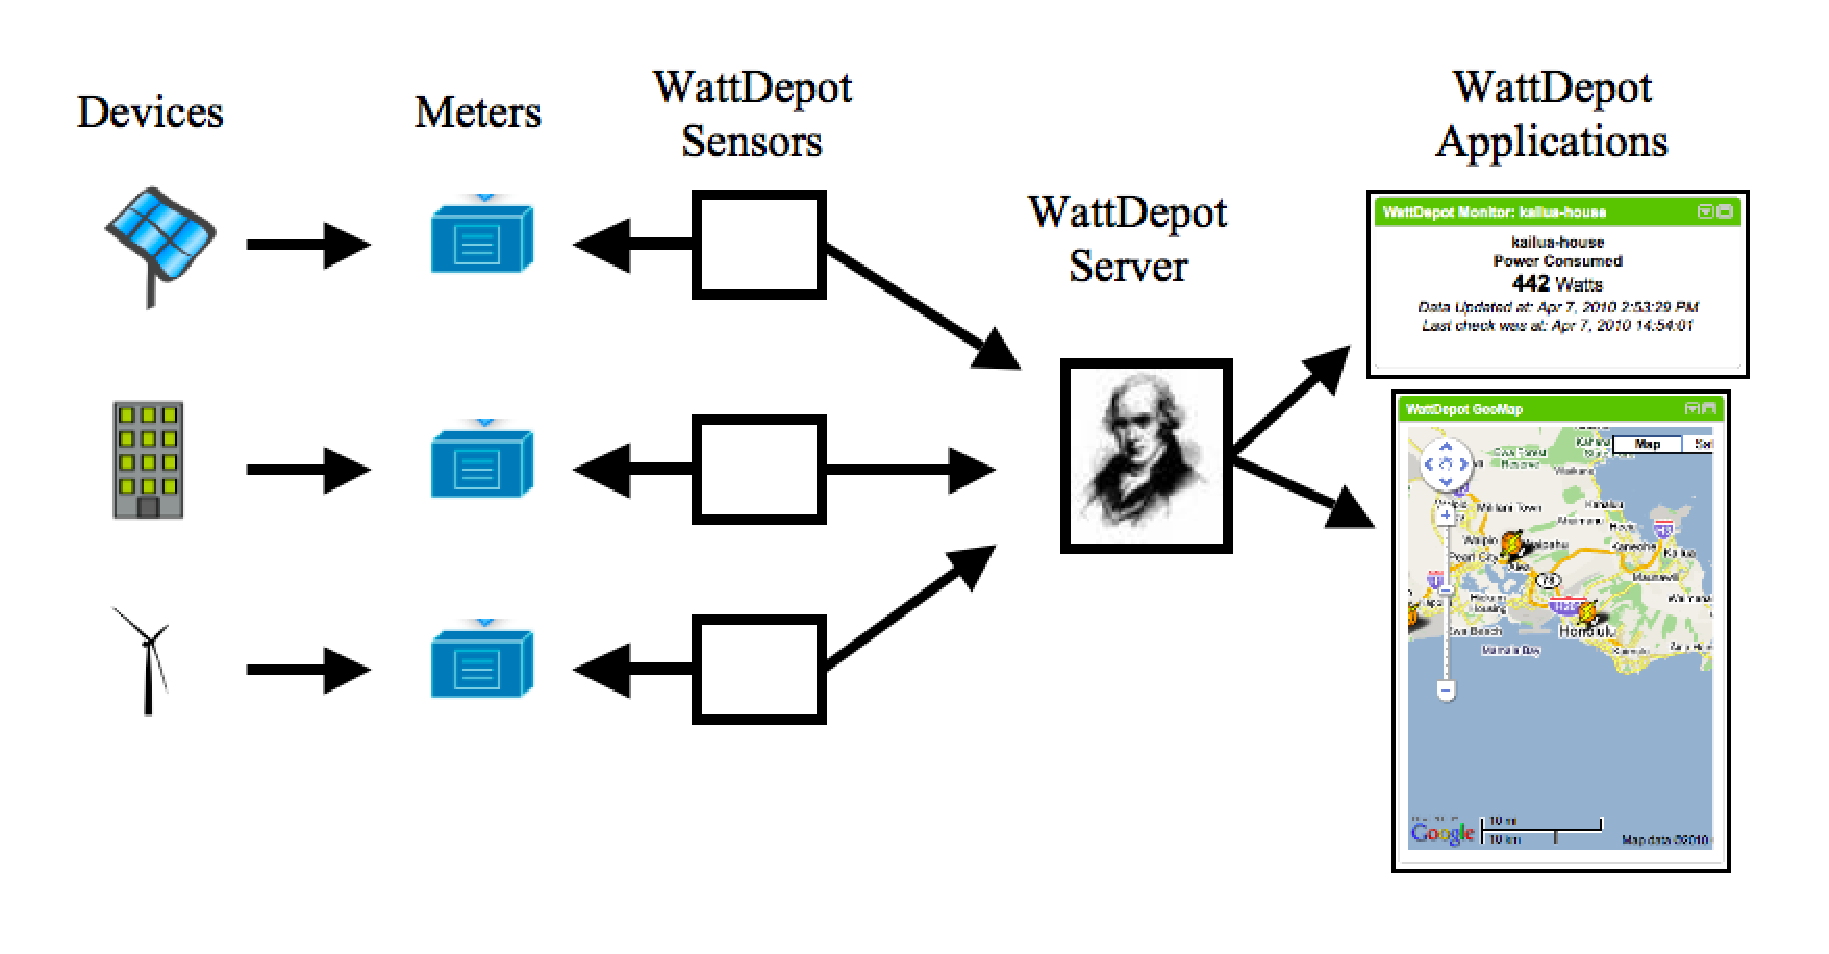
\includegraphics[width=0.8\textwidth]{architecture.eps}
  \caption{\em \small Architecture of WattDepot services}
  \label{fig:architecture}
\end{figure*} 


For example, consider a University that wants to implement a dorm energy
competition in which energy meters will be installed on each floor of the
dorm and residents of each floor will compete against each other to see who
can reduce their energy the most.  Prior to WattDepot, one could either buy a
proprietary, ``black box'' solution such as the Building Dashboard from
Lucid Design Group and be restricted to the set of meters and analyses they
support, or else start from scratch and build all of the energy data
collection, analysis, and visualization services.  WattDepot provides an
alternative approach, in which collection, storage, and analysis
capabilities are freely available and amenable to integration within a web
application developed by the user.  For those with some software
development capability, this can be a lower cost solution and/or support
customization beyond the ability of current proprietary solutions.

WattDepot services are designed at the ``enterprise'' scale as opposed to
the ``home'' or ``utility'' scales.  By home scale, we mean systems like
the TED 5000, which are designed to collect and analyze data about a single
residence, typically through a simple ``dashboard'' interface that runs on
the users local area network.  WattDepot is designed to collect, store, and
analyze data from a wider range of locations, and our performance analysis
tests indicate that it can easily process several thousand sensor data
storage requests per minute.  On the other hand, by utility scale, we mean
systems that can collect and store grid-level data comprising tens or
hundreds of thousands of residences, with revenue-grade measurement,
hardened storage, and security mechanisms.  WattDepot is not intended for
these more rigorous requirements.  We intend WattDepot to provide a
mechanism to accelerate innovative research and development into energy
analysis and visualization at the community level by providing an
extensible architecture and well documented, open source software platform.

The next section of this paper introduces the basic components of
WattDepot. Following this we describe some of our initial experiences with
the framework and conclude with our future directions. 

\section{WattDepot Services}

\subsection{Sensors}

{\em This section will describe how WattDepot sensors work and the kinds of
  WattDepot sensors that are currently under development.}

\subsection{Repositories}

{\em This section will describe the WattDepot repository, aspects of its
  REST API, its pluggable database backend design, and anything else of
  interest.}

\subsection{Clients}

{\em This section will talk about the various clients, including the CLI,
  the Wicket app, and the various google gadgets.}

\section{Applications}

{\em The section introduces how we are applying WattDepot at present. This
includes: the simulation of Oahu power plant generation to provide a kind
of ecotricity interface, and the Kukui Cup competition.}

\section{Future Directions}

{\em Micro-grids? Smart homes? Bayesian networks?}

\bibliographystyle{IEEEtran}
\bibliography{smartconsumer}
\end{document}











